\documentclass[tikz, margin=1mm]{standalone}

% fancy way of adding oriented arrows to path using various tikzlibraries
% taken from Tikz manual (see section 51.5.1)

%\usetikzlibrary {decorations.markings}
%\begin{tikzpicture}[decoration={
%markings,% switch on markings
%mark=between positions 0 and .75 step 4mm with {\arrow{stealth}},
%mark=between positions .75 and 1 step 4mm with {\arrowreversed{stealth}}}
%]
%\draw [help lines] grid (3,2);
%\draw [postaction={decorate}] (0,0) -- (3,1) arc (0:180:1.5 and 1);
%\end{tikzpicture}

\begin{document}
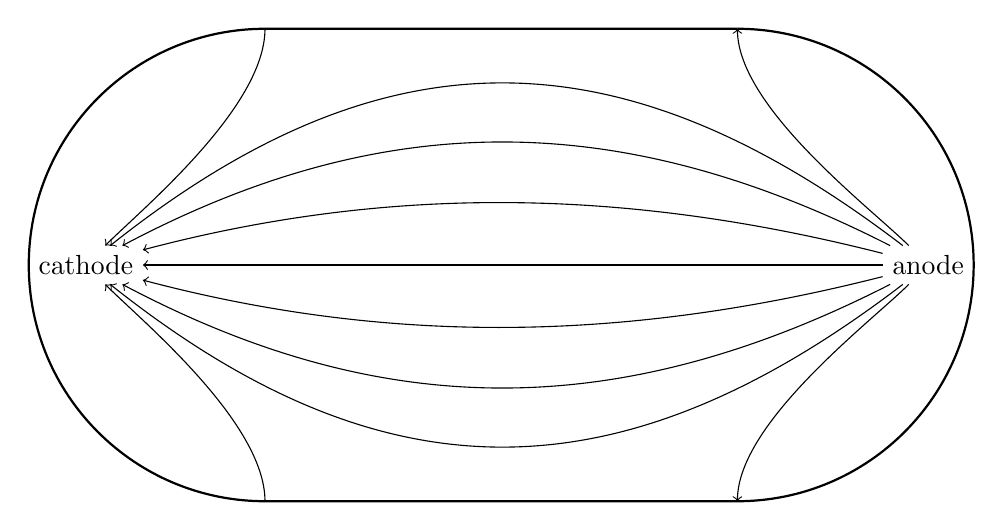
\begin{tikzpicture}

% arc construction
% 90 degree to right, -90 degree to left
% note that direction of arc drawing is anticlockwise, so negative angle != positive angle

\draw[thick] (3, 3) -- (-3, 3) arc (90:270:3);
\draw[thick] (-3, -3) -- (3,-3) arc (-90:90:3);
%\draw (-6,-6) rectangle (6,6);

\node[right] (c) at (-6,0) {cathode};
\node[left] (a) at (6,0) {anode};

\draw[<-] (c) -- (a);
% electrons flow from cathode to anode
% but (internal) current flows from anode to cathode

% see TikZ manual for special interpretation of relative coordinates for Bezier curves
\draw[<-] (c) .. controls (-1.5, -1) and (1.5, -1) .. (a);
\draw[<-] (c) .. controls (-1.5, -2) and (1.5, -2) .. (a);
\draw[<-] (c) .. controls (-1.5, -3) and (1.5, -3) .. (a);
\draw[<-] (c) .. controls +(315:1) and +(90:1) .. (-3, -3);
\draw[->] (a) .. controls +(225:1) and +(90:1) .. (3, -3);

% symmetric pairs
\draw[<-] (c) .. controls (-1.5, 1) and (1.5, 1) .. (a);
\draw[<-] (c) .. controls (-1.5, 2) and (1.5, 2) .. (a);
\draw[<-] (c) .. controls (-1.5, 3) and (1.5, 3) .. (a);
\draw[<-] (c) .. controls +(45:1) and +(270:1) .. (-3, 3);
\draw[->] (a) .. controls +(135:1) and +(270:1) .. (3, 3);

\end{tikzpicture}
\end{document}
